\subsection{Excercise DockerEnvironmentSetup}
This exercise sets up the Docker environment.
The goal is to install Docker and run the Hello-World container.

First, Docker is installed on the author's machine.
A quick verification is done to ensure that the installation was successful.
After that, the Hello-World container is run twice explaining the differences between the first and second execution.

\subsubsection*{Installing Docker}
The installation is carried out on the author's machine running Windows 11 with WSL2.
The installation is done by following the official Docker documentation \cite{DOC-INS} and the provided guide on the task sheet \cite{CM-G-BSD}.

After successfully installing Docker, the installation is verified by running \texttt{docker \-\-version} and \texttt{docker-compose \-\-version} in the terminal.
The output of the commands is shown in \autoref*{fig:docker_installation_verification}.

\begin{figure}
    \centering
    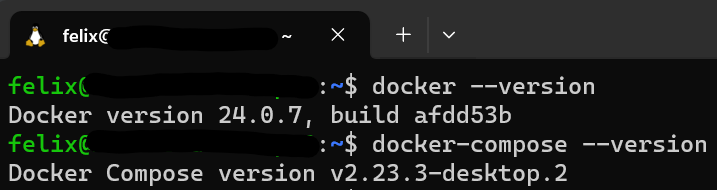
\includegraphics[width=0.8\textwidth]{figures/microservices/dmCar/ms_dmCar_dockerInstallation.png}
    \caption{Docker Installation Verification}
    \label{fig:docker_installation_verification}
\end{figure}
\subsubsection*{Running Hello-World Container}
The next step is to run the Hello-World container.
This is done by running the \texttt{docker run hello-world} command in the terminal.
The command is executed twice showing the differences between both executions.

Execution one is shown in \autoref*{fig:docker_hello_world_first_execution}.
The output shows that the image needed for the container is not available locally at first.
Therefore, the image is pulled automatically from the Docker Hub.
Afterwards, the container is started and the output is shown.

The second execution is shown in \autoref*{fig:docker_hello_world_second_execution}.
Here, the image is already available locally and therefore, no new image needs to be pulled from the Docker Hub.
The container is started instantly and the same output is shown.

\begin{figure}
    \centering
    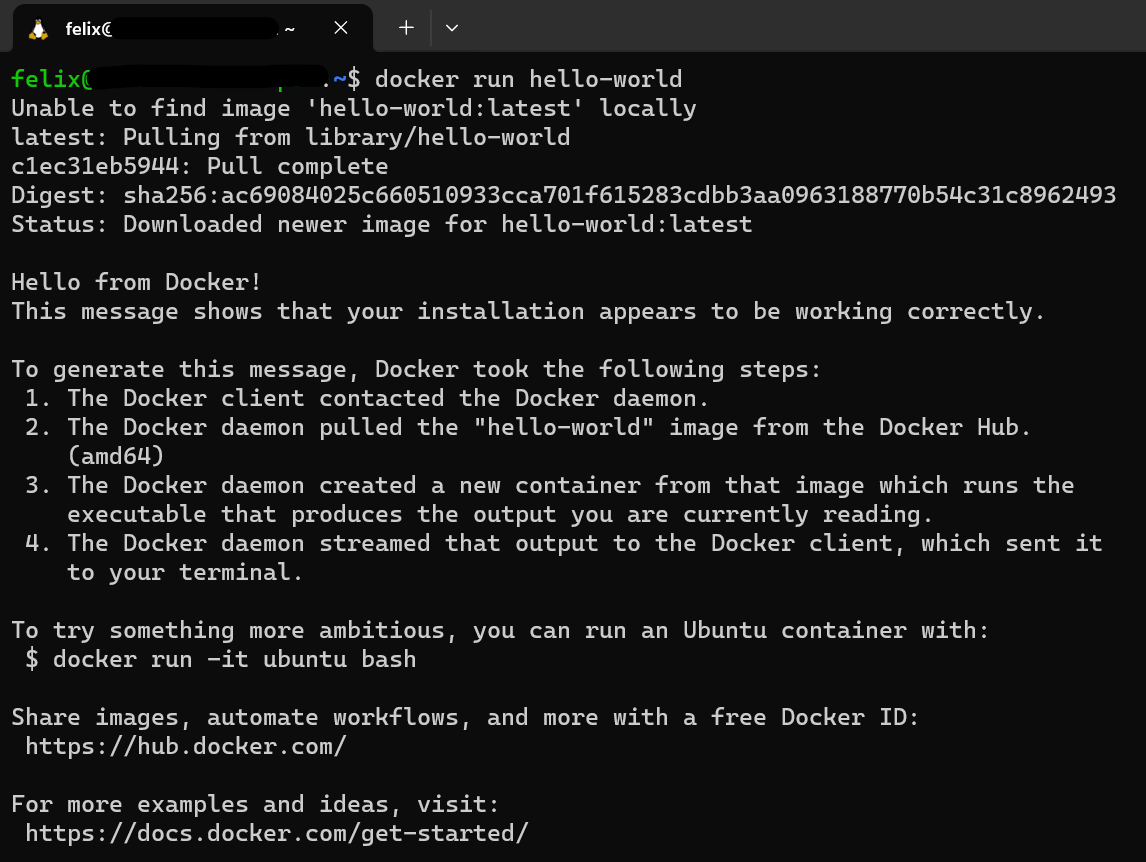
\includegraphics[width=0.6\textwidth]{figures/microservices/dmCar/ms_dmCar_dockerHelloWorldFirstExecution.png}
    \caption{First Execution of Hello-World Container}
    \label{fig:docker_hello_world_first_execution}
\end{figure}

\begin{figure}
    \centering
    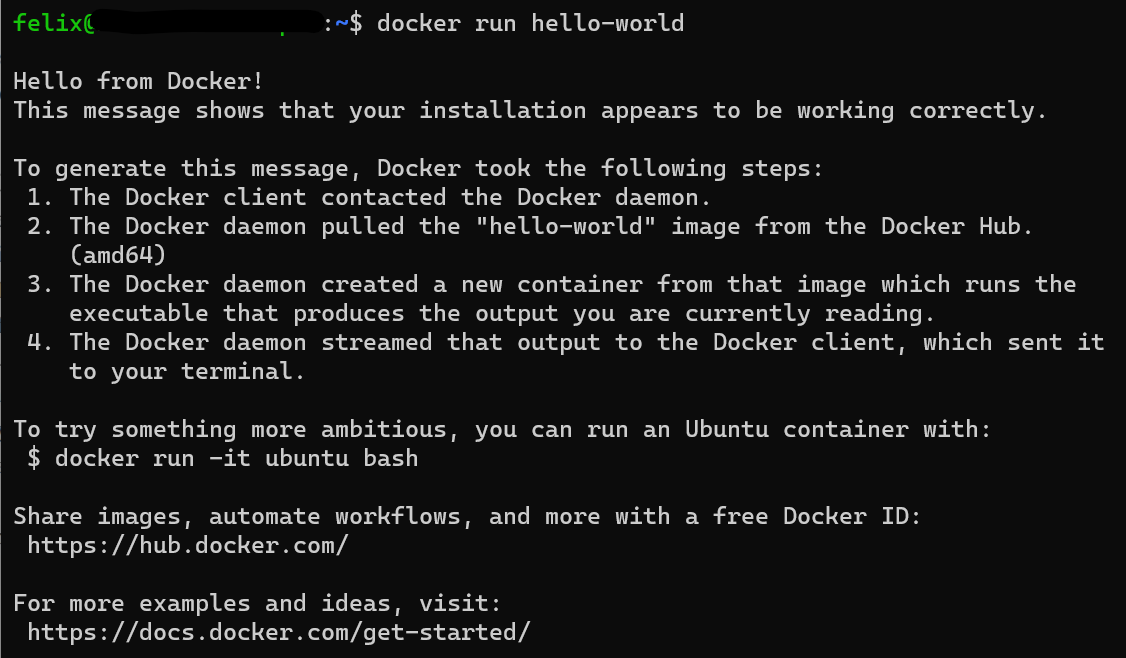
\includegraphics[width=0.6\textwidth]{figures/microservices/dmCar/ms_dmCar_dockerHelloWorldSecondExecution.png}
    \caption{Second Execution of Hello-World Container}
    \label{fig:docker_hello_world_second_execution}
\end{figure}

%==============================================================================

\subsection{Excercise DockerContainerization}
Docker is a containerization platform that allows for the creation, deployment, and execution of containers.
This exercise introduces containerization by implementing it on the DM-Car microservice.
This is done by creating a Dockerfile, building and optimizing a Docker image, and defining a \texttt{.dockerignore} file.
After this is done, the DM-Car application can be containerized by running the Docker image.

\subsubsection*{Add Dockerfile to DM-Car}
The first step is to add a Dockerfile to the DM-Car project.
This is done by creating a new file called \texttt{Dockerfile} in the root directory of the project.
The content of the file is copied from the Golang project template located at \texttt{1.EngineeringKnowledge/CICD/GolangTemplate}.
After that, the content is pushed to the GitLab repository.

\subsubsection*{Familiarize With Dockerfile Syntax}
The \texttt{dockerfile} is separated into three distinct stages: build, test, and production.
This task analyzes each of them and explains their purpose.
Also, the functionality of the used instructions is explained.

\paragraph*{Build Stage}
The code of the build stage is shown in \autoref*{lst:build_stage_dm_car}.

The build stage builds the go project.
It checks and downloads dependencies, copies and compiles the source code and creates an executable file called \texttt{main}.
This stage, therefore, is the primitive for the following stages.
 
\begin{lstlisting}[
    style=kit-cm,
    caption={Build Stage of the Dockerfile},
    label={lst:build_stage_dm_car},
    float=h
    ]
# ==================
# BUILD STAGE
# ==================
FROM golang:1.21.0-alpine3.18 AS build  # defines the base image that is used for this stage

WORKDIR /app                            # sets the working directory in the container
COPY /src/go.mod /src/go.sum ./         # copies the go.mod and go.sum files from the source directory to the working directory
RUN go mod download                     # runs the go mod download command to download the dependencies
COPY /src/ ./                           # copies the source code from the src directory to the working directory
RUN go build -o main .                  # compiles the source code and creates an executable file called main
\end{lstlisting}

\paragraph*{Test Stage}
The code of the test stage is shown in \autoref*{lst:test_stage_dm_car}.

This stage uses the code from the previous build stage and runs tests on it.
By running it before the production stage integrity of the code is ensured.
If the tests fail, production can be stopped and the code can be fixed ensuring that only working code makes it to the production stage.

\begin{lstlisting}[
    style=kit-cm,
    caption={Test Stage of the Dockerfile},
    label={lst:test_stage_dm_car},
    float=h
    ]
# ==================
# TEST STAGE
# ==================
FROM build AS test      # defines the base image, which is the build stage

RUN go test -v ./...    # runs the 'go test' command to run all tests in the project
\end{lstlisting}

\paragraph*{Production Stage}
The code of the production stage is shown in \autoref*{lst:production_stage_dm_car}.

This is the final production stage.
It uses the \texttt{alpine} image as a base image and copies the essential artifacts from the test stage, which is the main executable, into the production image.
This image only contains the essential artifacts needed to correctly run the application.

\begin{lstlisting}[
    style=kit-cm,
    caption={Production Stage of the Dockerfile},
    label={lst:production_stage_dm_car},
    float=h
    ]
# ==================
# PRODUCTION STAGE
# ==================
FROM alpine:3.18 AS production  # defines the base image, which is the alpine image
                                # the image is then called 'production'

WORKDIR /root/                  # sets the working directory in the container
COPY --from=test /app/main .    # copies the main executable from the test stage to the working directory
EXPOSE 80                       # exposes port 80, which is used by the application
CMD ["./main"]                  # runs the main executable
\end{lstlisting}

\paragraph*{Wrap Up}
The Dockerfile is now complete.
It contains all the necessary stages to build, test, and run the DM-Car application.
The stages are arranged in a way that the build stage is executed first, then the test stage, and finally the production stage.
This ensures that only working code is deployed to the production stage.

Now, the Dockerfile will be used to build a Docker image.

\subsubsection*{Build Docker Image}
The Docker image is built by running \texttt{docker build -t dm-car:base .} in the project's root directory.

% Explain the parameters
\texttt{docker build} builds an image from a Dockerfile and a context with the context being the provided path or URL linked to a set of files.
The image provides the necessary artifacts to run the application.
This can be, for example, the file system, dependencies, environment variables, and more.
The \texttt{\-t} flag is used to tag the image with a name and an optional tag in the \texttt{name:tag} format.
In the case of the provided \texttt{docker build -t dm-car:base .} command, the image is tagged with the name \texttt{dm-car} and the tag \texttt{base}.
The context is set to the current directory in which the Dockerfile is located and, therefore the root directory of the project.

After running the command we can find the image by running the \texttt{docker image} command in the terminal.
The output is shown in \autoref{fig:docker_image}.

% What would happen without the flags and the dot
Just running \texttt{docker build} without any flags or arguments would result in an error.
Therefore \texttt{docker build .} is the minimum command to build an image.
It builds the image from the Dockerfile located in the current directory.
After the building process, the image is given the name \texttt{sha256:} followed by a hash.
Therefore the image can only be referenced by its hash, which is not very convenient.
The image also cannot be found using the \texttt{docker image} command.

\begin{figure}
    \centering
    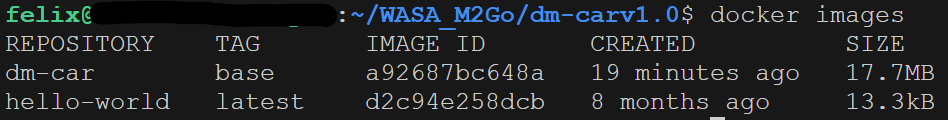
\includegraphics[width=0.7\textwidth]{figures/microservices/dmCar/ms_dmCar_dockerImages.png}
    \caption{Docker Image}
    \label{fig:docker_image}
\end{figure}

\subsubsection*{Build Optimized Image}
After optimizing the Dockerfile, the image is built again.
The new Dockerfile receives the same name of \texttt{dm-car} and the tag \texttt{optimized}.
Opening Docker Desktop and looking at the images, there are now two images with the same name but different tags.
The output is shown in \autoref{fig:docker_image_comparison}.

Comparing both images, the optimized image is about 1.7 MB smaller than the base image.
Also, the build time is reduced by about 3 seconds.

Therefore the optimized image is better suited for production.

\begin{figure}
    \centering
    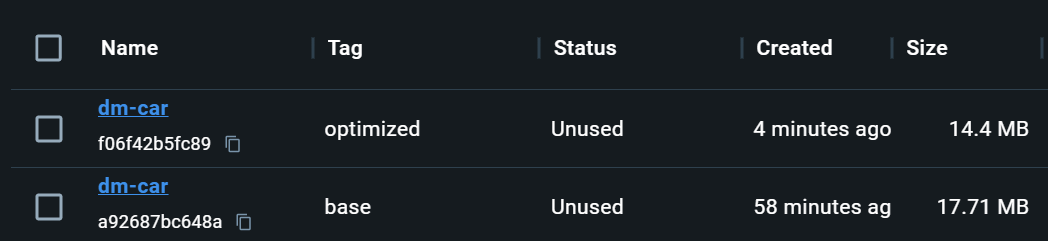
\includegraphics[width=0.7\textwidth]{figures/microservices/dmCar/ms_dmCar_optimizedComparison.png}
    \caption{Comparison of both Docker Images}
    \label{fig:docker_image_comparison}
\end{figure}

\subsubsection*{Define a File .dockerignore}
The \texttt{.dockerignore} file is used to exclude files and directories when running the \texttt{COPY} instruction.
This is useful to reduce the size of the context and therefore the size of the image.
The content of the file is shown in \autoref*{lst:dockerignore_file}.
It excludes the \texttt{specification} folder holding the API specification, the git directory, the \texttt{.gitignore} file, all markdown files, the cache directory, and the Dockerfile itself.
Furthermore, the \texttt{figures} and \texttt{pages} directories are excluded, which hold the images and the documentation of the project.
Therefore, only the necessary files for the execution are copied into the image.

\begin{lstlisting}[
    style=kit-cm,
    caption={.dockerignore File},
    label={lst:dockerignore_file},
    float=h
]
# files
Dockerfile
*.md
.gitignore

# folders
figures/
pages/
.git
.cache
src/controller/specification
\end{lstlisting}

\subsection{Excercise DockerCompose}
Docker Compose \cite{DOC-COM} is a tool for defining and running multi-container Docker applications.
It is used in this exercise to start the DM-Car application.
First, the familiarization with Docker Compose is done.
Then, the \texttt{dm-car} service is extended with a Postgres database.
After that, health checks are initialized to ensure the database is fully operational before the \texttt{dm-car} service starts.
Finally, the Postgres database is extended with persistent storage implemented using a named volume.

\subsubsection*{Familiarize with Docker Compose}
\texttt{docker compose} is a tool for defining and running multi-container Docker applications.
It uses a YAML file to configure the application's services.
Then, with a single command, the application's services are created and started.
This makes it easy to start a multi-container application with a single command.

Within the local deployment phase of the project, \texttt{docker compose} is used to start the DM-Car application.
After executing the command, the application is running and can be accessed via \texttt{http://localhost:80}.
Without \texttt{docker compose}, the application would have to be started manually by running the Docker image with the ports exposed and the environment variables set.
This is not only more time-consuming but also more error-prone.
Therefore \texttt{docker compose} is a useful tool for local development.

\subsubsection*{Extend DM-Car Docker Compose File With a Database}
The Postgres database using the \texttt{postgres:15.4} image is added to the Docker Compose file.
To configure the database, environment variables are used. \\
These are \texttt{POSTGRES\_HOST}, \texttt{POSTGRES\_USER}, \texttt{POSTGRES\_PASSWORD}, \texttt{POSTGRES\_PORT}, and \texttt{POSTGRES\_DATABASE}.
Setting all these variables is necessary to connect to the database.
Therefore, these values are added to the \texttt{dm-car} service in the Docker Compose file to ensure the correct connection variables are set.
The passwort also needs to be set in the \texttt{postgres} service.
\autoref*{lst:docker_compose_postgres} shows the changes made to the Docker Compose file.

After rerunning "\texttt{docker-compose up}" the \texttt{postgres} service is started additionally to the \texttt{dm-car} service.
This happens automatically because the \texttt{postgres} service is defined in the Docker Compose file.
In Docker Desktop, the running containers can be seen in the \texttt{dm-carv1.0} tab.
Both containers are running, the \texttt{dm-car}, which has port 80 exposed, and the \texttt{postgres} container.
This can be seen in \autoref*{fig:docker_compose_up}.

\paragraph*{Importance of Segregating Configuration from Application Logic:}
Configuration and application logic are distinct concepts of a software system.
Both serve a different purpose.
While configuration logic is used to set parameters and values on how a system's components are structured, application logic is used to implement the system's functionality.
Therefore it is important to segregate configuration from application logic due to the SoC principle.
Also, it ensures readability of the code and therefore makes it easier to maintain.

\begin{lstlisting}[
    style=kit-cm,
    caption={Added Postgres Service to Docker Compose File},
    label={lst:docker_compose_postgres},
    float=h
]
...
services:
  dm-car:
    ...
    depends_on:
      postgres:
        condition: service_healthy
    environment:
      - POSTGRES_HOST=postgres
      - POSTGRES_USER=postgres
      - POSTGRES_PASSWORD=password
      - POSTGRES_PORT=5432
      - POSTGRES_DATABASE=postgres
  postgres:
    image: postgres:15.4
    ...
    environment:
      - POSTGRES_PASSWORD=password
    volumes:
      - ./postgres-data:/var/lib/postgresql/data
\end{lstlisting}

\begin{figure}
    \centering
    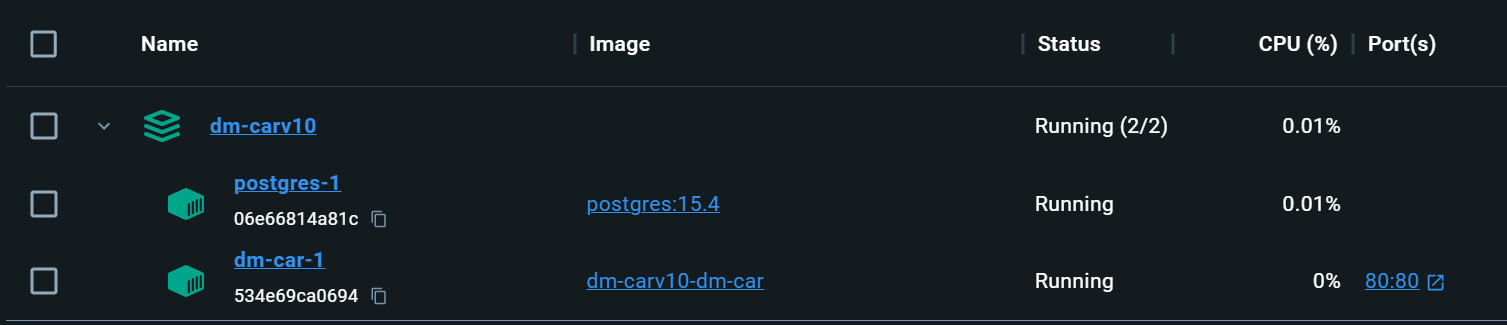
\includegraphics[width=0.8\textwidth]{figures/microservices/dmCar/ms_dmCar_dockerComposePostgres.png}
    \caption{Docker Desktop after running \texttt{docker-compose up}}
    \label{fig:docker_compose_up}
\end{figure}

\subsubsection*{Implement Health Check for Database Initialization}
Two sections are added to the Docker Compose file to fulfill this task.
The changes are shown in \autoref*{lst:docker_compose_health_check}.

% Changes on dm-car service
First, the \texttt{depends\_on} section is added to the \texttt{dm-car} service.
It ensures, that the \texttt{postgres} service is started before the \texttt{dm-car} service.
Next, the \texttt{environment} section is added to the \texttt{dm-car} service containing the \texttt{CONDITION} variable.
The environment section in general defines environment variables for the service.
In this case, the \texttt{CONDITION} variable is set to \texttt{service\_healthy}.
This ensures, that the \texttt{dm-car} service is only started if the \texttt{postgres} service is healthy.

% Changes on Postgres service
The \texttt{postgres} service receives a health check by adding the \texttt{healthcheck} section.
A health check defines how a container can be tested if it is working correctly.
With no health checks defined, Docker assumes that the container is healthy and starts it whether it is or not.
\texttt{test} defines the command that will be executed.
It is the health check of the container.
The following attributes specify the tests to be executed in 10-second intervals, trying three times before giving up and waiting for a total of 30 seconds for a return code before declaring the health check as failed.

% Discuss the significance of ensuring the service is fully operational before another dependant service starts
Ensuring one service is fully operational before starting another dependent service is very significant.
If the \texttt{dm-car} service is started before the \texttt{postgres} service, the \texttt{dm-car} service will fail to start.
It needs to connect to the database to run correctly.
Therefore, the \texttt{postgres} service needs to be started first.
Also, by starting one service after another, race conditions can be prevented.
This might happen if both services access the same resources.
Furthermore, issues due to partial failures can be avoided.
Services that depend on other services yet start before them might work with incomplete information.
This can lead to unexpected behavior and errors.
This also enables the efficient utilization of resources.
The deployment of services can therefore be optimized.

% How does this contribute to the microservice paradigm
Ensuring system reliability and resilience by ensuring one service is fully operational before another dependent service is crucial in the microservice paradigm.
When applications are composed of loosely coupled and independently deployable services, dependencies are common.
If a dependent service starts before the required service is fully operational it may encounter errors or false behavior, which may in return lead to service disruptions.

\begin{lstlisting}[
    style=kit-cm,
    caption={Added Health Checks to Docker Compose File},
    label={lst:docker_compose_health_check},
    float=h
]
services:
    dm-car:
        ...
        depends_on:
          postgres:
            condition: service_healthy
postgres:
    ...
    healthcheck:
        test: pg_isready -U postgres
        interval: 10s
        timeout: 30s
        retries: 3
\end{lstlisting}

\subsubsection*{Extend Postgres Database With Persistent Storage}
A volume in general is a mechanism for persisting data generated and used by Docker containers.
These volumes are completely managed by Docker and exist outside the containers' lifecycle.
Therefore volumes can be safely shared among multiple containers, they are easy to back up or migrate, and they do not increase the size of the containers using it.
A named volume is a type of volume that has been given a specific name.

% Code changes
The code changes adding a named volume to the \texttt{postgres} service in the \texttt{docker-compose} file are shown in \autoref*{lst:docker_compose_named_volume}.
The volume is called \texttt{postgres-data} and is mounted to the \texttt{/var/lib/postgresql/data} directory of the \texttt{postgres} service.
This directory is used by Postgres to store its data persistently.

% Importance of backing services in stateless services
Stateless services, in contrast to stateful services, do not store any client state on the server between requests.
This means that every request is independent of the previous one.
Therefore, the service relies on backing services to manage and persist its data.
Furthermore, using backing services makes sure critical information is not lost between service restarts or failures.
This enables a certain degree of fault tolerance.
Also, backing services can be scaled independently of the service itself.
This allows for a more efficient utilization of resources.
Therefore the overall performance, maintainability, and scalability of the stateless service can be improved.

\begin{lstlisting}[
    style=kit-cm,
    caption={Code to Add a Named Volume to the Postgres Service},
    label={lst:docker_compose_named_volume},
    float=h
]
...
services:
  ...
  postgres:
    ...
    volumes:
      - ./postgres-data:/var/lib/postgresql/data
\end{lstlisting}